\documentclass[tikz]{standalone}
\usepackage{tikz}
\usepackage{siunitx}
\DeclareSIUnit\degF{\text{°}F}

\definecolor{codeblue}{RGB}{69, 161, 248}
\definecolor{codegray}{RGB}{40, 40, 40}
\usetikzlibrary{shapes,arrows}
\tikzstyle{decision} = [diamond, draw, fill=codegray, text=white,
    text width=4.5em, text badly centered, node distance=3cm, inner sep=0pt]
\tikzstyle{block} = [rectangle, draw, fill=codeblue,  text=white,
    text width=5em, text centered, rounded corners, minimum height=4em]
\tikzstyle{line} = [draw, -latex']


\begin{document}
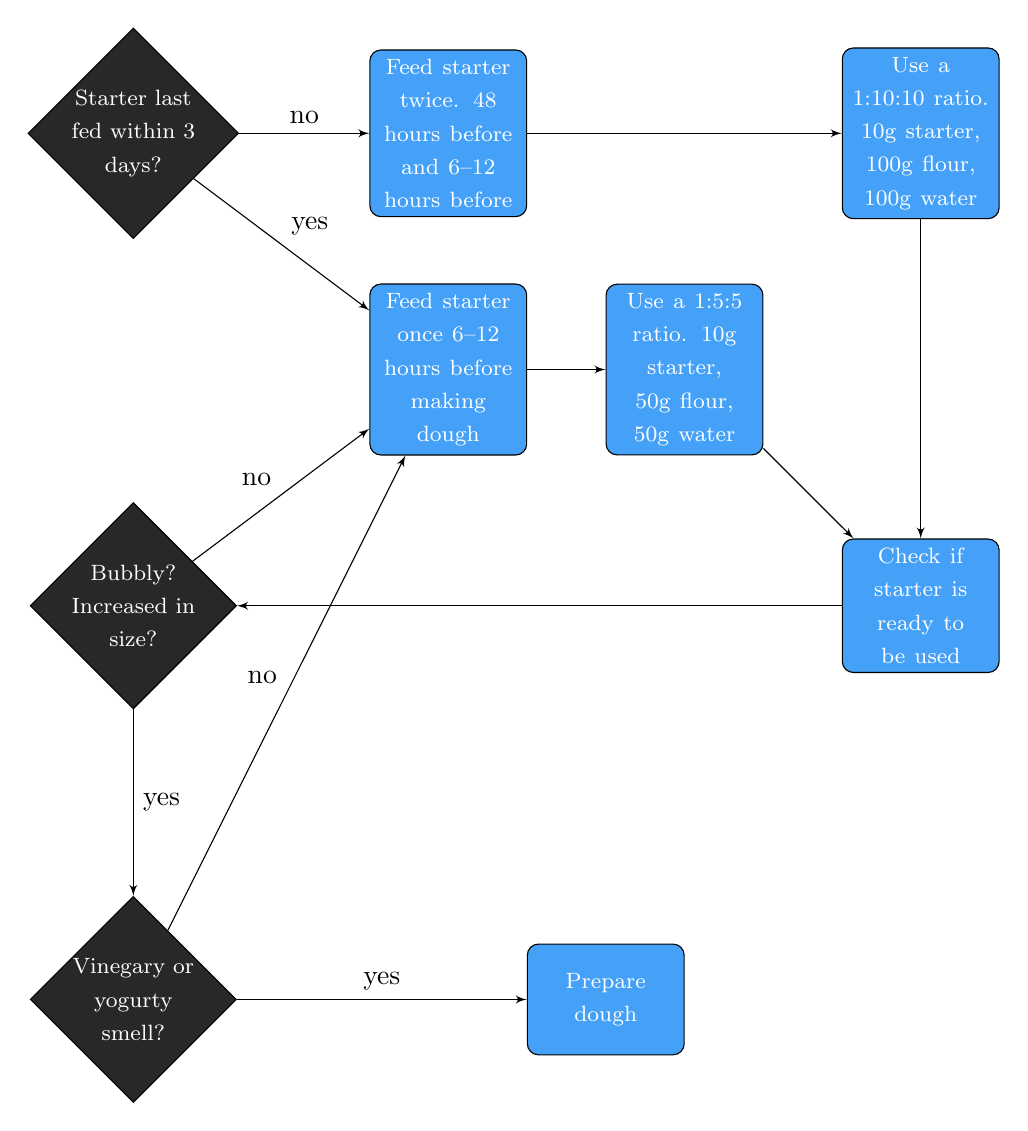
\begin{tikzpicture}[node distance = 3cm, auto]
  \node [decision] (init) {\footnotesize Starter last fed within 3 days?};
  \node [block, right of=init, node distance=4cm] (feed_no_branch)
    {\footnotesize Feed starter twice. 48 hours before and 6--12 hours before};
  \node [block, below of=feed_no_branch, node distance=3cm] (feed_yes_branch)
    {\footnotesize Feed starter once 6--12 hours before making dough};
  \node [block, right of=feed_no_branch, node distance=6cm] (high_ratio)
    {\footnotesize Use a 1:10:10 ratio. 10g starter, 100g flour, 100g water};
  \node [block, right of=feed_yes_branch, node distance=3cm] (low_ratio)
    {\footnotesize Use a 1:5:5 ratio. 10g starter, 50g flour, 50g water};
  \node [block, below of=high_ratio, node distance=6cm] (check_starter)
    {\footnotesize Check if starter is ready to be used};
  \node [decision, below of=init, node distance=6cm] (size_check)
    {\footnotesize Bubbly? Increased in size?};
  \node [decision, below of=size_check, node distance=5cm] (smell_check)
    {\footnotesize Vinegary or yogurty smell?};
  \node [block, right of=smell_check, node distance=6cm] (make_dough)
    {\footnotesize Prepare dough};
  \path [line] (init) -- node{no} (feed_no_branch);
  \path [line] (init) -- node{yes} (feed_yes_branch);
  \path [line] (feed_yes_branch) -- (low_ratio);
  \path [line] (feed_no_branch) -- (high_ratio);
  \path [line] (high_ratio) -- (check_starter);
  \path [line] (low_ratio) -- (check_starter);
  \path [line] (check_starter) -- (size_check);
  \path [line] (size_check) -- node{no} (feed_yes_branch);
  \path [line] (size_check) -- node{yes} (smell_check);
  \path [line] (smell_check) -- node{no} (feed_yes_branch);
  \path [line] (smell_check) -- node{yes} (make_dough);
\end{tikzpicture}
\end{document}
